% !TeX spellcheck = en_US
% !TeX root = ../../build/architecture.tex
% !TeX TXS-program:compile = txs:///xelatex/[--shell-escape]


\renewcommand{\mytitle}{Basic Principles of the Polygon zkEVM Proving System}
\ifZEROSEC \fi
\ifSEC \section{\mytitle{}}\fi
\ifSUBSEC \subsection{\mytitle{}}\fi
\ifSUBSUBSEC \subsubsection{\mytitle{}}\fi


\ifARCHMAP
\begin{frame}{Architecture of the zkEVM: Prover and Executor}
\begin{figure}
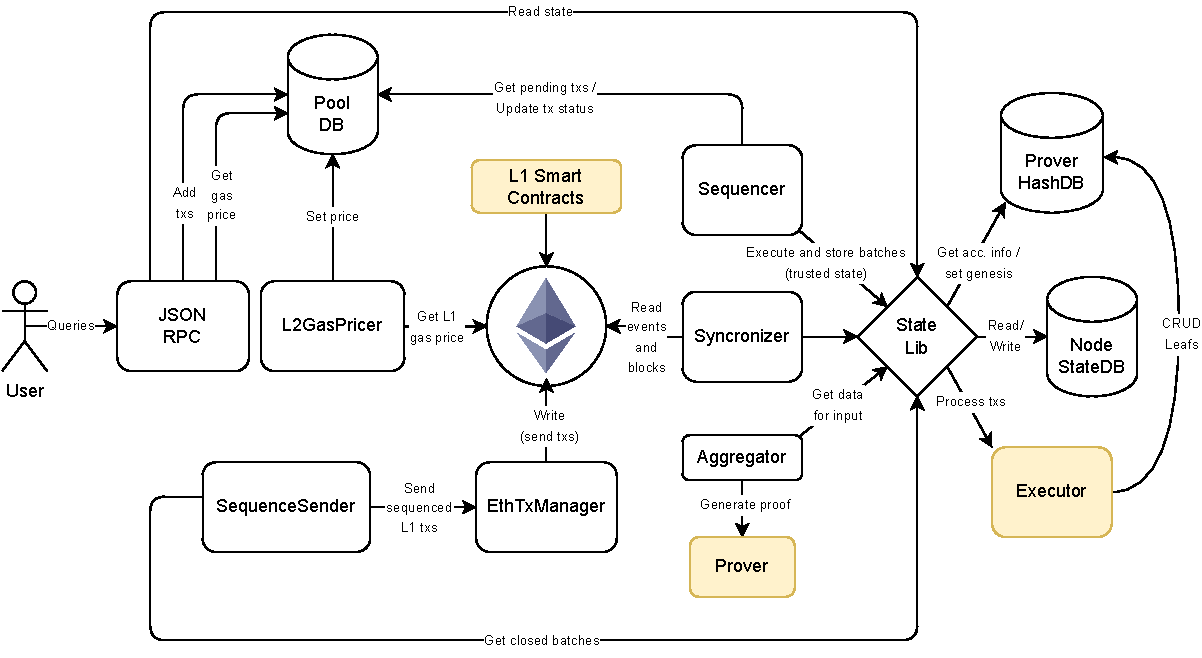
\includegraphics[width=0.85\columnwidth]{\zkevmdir/figures/architecture/intro-proving-system/architecture-map-prover-executor.drawio}
\end{figure}
\end{frame}



\begin{frame}{List of To Be Covered Concepts}
\begin{columns}
\begin{column}{0.48\textwidth}
\begin{itemize}
\item Provers. \hfill \Square
\item Execution trace. \hfill \Square
\item Witness and fixed columns. \hfill \Square
\item Executors (general purpose and computation-specific). \hfill \Square
\item zk Assembly. \hfill \Square
\item ROM of the zkEVM. \hfill \Square
\item forkId. \hfill \Square
\end{itemize}
\end{column}
\begin{column}{0.48\textwidth}
\begin{itemize}
\item PIL (Polynomial Identity Language). \hfill \Square
\item PIL2 (WIP). \hfill \Square
\item Publics and privates. \hfill \Square
\item Verifiers (Fflonk). \hfill \Square
\item Selector columns. \hfill \Square
\item zkEVM compatibility/equivalence types. \hfill \Square
\item Secondary execution matrices A.K.A state machines. \hfill \Square
\item PIL namespaces. \hfill \Square
\item State machine interconnection with lookups. \hfill \Square
\end{itemize}
\end{column}
\end{columns}
\end{frame}
\fi



\begin{frame} {Functions of the L2 Prover}
\begin{block}{Prover}
The "Prover" is a component whose main goal is to generate a \textbf{proof} that for the correct execution of a given program with an specific set of inputs. The proving process is a resource-consuming process.
\end{block}

\begin{figure}

\includegraphics[width=0.7\columnwidth]{\zkevmdir/figures/architecture/intro-proving-system/goal-prover.drawio}
\end{figure}

\begin{columns}
\begin{column}{0.7\textwidth}
\begin{itemize}
\item To generate such a proof, we first need to create an \textbf{execution trace}.
\item An execution trace is just a \textbf{matrix} (or grid) of cells with rows and columns.
\end{itemize}
\end{column}
\begin{column}{0.3\textwidth}
$$
\begin{array}{|c|c|c|c|c|}
\hline
 &  & & & \\ \hline
 &  & & &\\ \hline
 &  & & &\\ \hline
 &  & & &\\ \hline
\end{array}
$$
\end{column}
\end{columns}
\end{frame}




\begin{frame}[allowframebreaks]{Execution Trace Example}
\begin{itemize}
\item Let $x=(x_0, x_1, x_2)$ a vector of given inputs.
\item We want to implement an execution trace for the following computation:
$$[(x_0+x_1)\cdot4]\cdot x_2$$
\item Suppose that we only have the following operations available:
  \begin{enumerate}
  \item Copy inputs into cells of the execution trace.
  \item Sum two cells of the same row, and leave the result in a cell of the next row (\texttt{ADD}).
  \item Multiply by a constant, and leave the result in a cell of the next row (\texttt{TIMES4}).
  \item Multiply two cells of the same row, and leave the result in a cell of the next row (\texttt{MUL}).
  \end{enumerate}
\item Let's consider that our execution trace has $3$ columns and a bounded number of rows (so that we can fit the needed computation in it):
$$
\begin{array}{|c|c|c|}
\hline
\textbf{A} & \textbf{B} & \textbf{C} \\ \hline
a_0 & b_0 & c_0 \\ \hline
a_1 & b_1 & c_1 \\ \hline
... & ... & ...\\ \hline
a_n & b_n & c_n \\ \hline
\end{array}
$$
\item The columns of an execution trace are often called \textbf{registers} (so we may name them interchangeably).
\end{itemize}


\framebreak
\begin{itemize}
\item Suppose we are given the following inputs $x=(x_0, x_1, x_2)=(1,2,5)$.
\item We can model our desired computation $[(x_0+x_1)\cdot4]\cdot x_2$ to fit our execution trace using only the available operations as follows:
\end{itemize}

\vspace{0.3cm}
\begin{large}
\begin{table}[h!]
\centering

\begin{tabular}{|c|c|c|}
\hline
\textbf{A} & \textbf{B} & \cellcolor{lightgray} \textbf{C} \\ \hline
1 & 2 & \cellcolor{lightgray} \\ \hline
3 & & \cellcolor{lightgray} 4 \\ \hline
12 & 5 & \cellcolor{lightgray} \\ \hline
60 & & \cellcolor{lightgray} \\ \hline
\end{tabular}
\hspace{1mm}
\begin{tabular}{r}
                    \\
$[a_0=x_0, b_0=x_1]$  \\
                    \\
$[b_2 = x_2]$         \\
                    \\

\end{tabular}
\hspace{1em}
\begin{tabular}{l}
                    \\
\texttt{ADD} \\
\texttt{TIMES4} \\
\texttt{MUL} \\
\\
\end{tabular}
\end{table}
\end{large}
\end{frame}





\begin{frame}{Witness and Fixed Columns}
\begin{itemize}
\item Notice that if we change the inputs $x=(x_0, x_1, x_2)=(5,3,2)$, we can perform exactly the same computation as before but the execution trace changes (most of) its values \textbf{but not its shape}.
$$
\begin{array}{|c|c|c|}
\hline
\textbf{A} & \textbf{B} & \cellcolor{lightgray} \textbf{C} \\ \hline
5 & 3 & \cellcolor{lightgray} \\ \hline
8 & & 4 \cellcolor{lightgray} \\ \hline
32 & 2 & \cellcolor{lightgray} \\ \hline
64 & & \cellcolor{lightgray} \\ \hline
\end{array}
$$

\item The columns that depend on the input (in this case A and B) are called \textbf{witness columns}.
\item The columns that are the same for all inputs (in this case column C) are known as \textbf{fixed columns} (which we will mark in gray color).
\item Note that fixed columns don't change as they are an intrinsic part of the computation.
\end{itemize}
\end{frame}






\begin{frame}{Functions of the Executor}

\begin{block}{Executor}
The "Executor" is a component whose main purpose is to generate a (correct) execution trace from a given set of inputs.
\end{block}

\begin{figure}
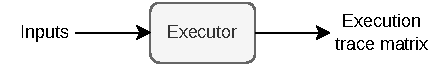
\includegraphics[width=0.65\columnwidth]{\zkevmdir/figures/architecture/intro-proving-system/general-executor}
\end{figure}
\end{frame}




\begin{frame} [allowframebreaks] {How to implement the Executor}
\textbf{Approach \#1:}
    \begin{itemize}
    \item As a component that runs just one given computation.
    \item Application Specific Integrated Circuit (ASIC) as electronic analogy: an ASIC
    is a circuit specifically designed to run, very efficiently, a single computation.
    \item We also call this executor a \textbf{native executor}.
    \end{itemize}

\begin{figure}
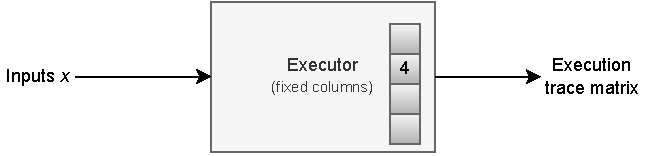
\includegraphics[width=0.9\columnwidth]{\zkevmdir/figures/architecture/intro-proving-system/executor-asic-approach.drawio}
\end{figure}


\framebreak
\textbf{Approach \#2:}
\begin{itemize}
\item As a general purpose processor, which means as a component that can run several computations or "programs".
\item In this case, the executor is as follows:
\end{itemize}
\begin{figure}[H]
\centering
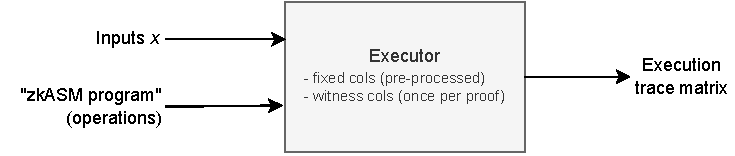
\includegraphics[width=0.9\columnwidth]{\zkevmdir/figures/architecture/intro-proving-system/executor-cpu-approach.drawio}
\end{figure}
\end{frame}





\begin{frame} {Example of an Executor that Reads Assembly Programs}
\large
Using an executor that reads assembly, we could run two zkASM programs:
\normalsize
~\\
\begin{columns}
\begin{column}{0.55\textwidth}
\textbf{Program 1: $[(x_0+x_1)\cdot4]\cdot x_2$} having $x=(x_0, x_1, x_2)=(1,2,5)$ as inputs.

\vspace{1em}

\begin{table}[h!]
\centering

\begin{tabular}{|c|c|c|}
\hline
\textbf{A} & \textbf{B} & \cellcolor{lightgray} \textbf{C} \\ \hline
1 & 2 & \cellcolor{lightgray} \\ \hline
3 & & \cellcolor{lightgray} 4 \\ \hline
12 & 5 & \cellcolor{lightgray} \\ \hline
60 & & \cellcolor{lightgray} \\ \hline
\end{tabular}
\hspace{1mm}
\begin{tabular}{r}
                    \\
$[a_0=x_0, b_0=x_1]$  \\
                    \\
$[b_2 = x_2]$         \\
                    \\

\end{tabular}
\hspace{1em}
\begin{tabular}{l}
                    \\
\texttt{ADD} \\
\texttt{TIMES4} \\
\texttt{MUL} \\
\\
\end{tabular}
\end{table}
\end{column}
\begin{column}{0.45\textwidth}
\textbf{Program 2 $(x_0\cdot16)\cdot x_1$} having $x=(x_0, x_1)=(2, 3)$ as inputs.

\vspace{1em}

\begin{table}[h!]
\centering

\begin{tabular}{|c|c|c|}
\hline
\textbf{A} & \textbf{B} & \cellcolor{lightgray} \textbf{C} \\ \hline
2 &  & \cellcolor{lightgray} 4\\ \hline
8 & & \cellcolor{lightgray} 4 \\ \hline
32 & 3 & \cellcolor{lightgray} \\ \hline
96 & & \cellcolor{lightgray} \\ \hline
\end{tabular}
\hspace{1mm}
\begin{tabular}{r}
                    \\
$[a_0=x_0]$  \\
                    \\
$[b_2 = x_1]$         \\
                    \\

\end{tabular}
\hspace{1em}
\begin{tabular}{l}
                    \\
\texttt{TIMES4} \\
\texttt{TIMES4} \\
\texttt{MUL} \\
\\
\end{tabular}
\end{table}
\end{column}
\end{columns}

\footnotesize
\url{https://github.com/0xPolygonHermez/zkevm-rom}
\normalsize
\end{frame}




%TODO WIP
\begin{frame}{Single-computation vs General-computation Executor}
\begin{figure}
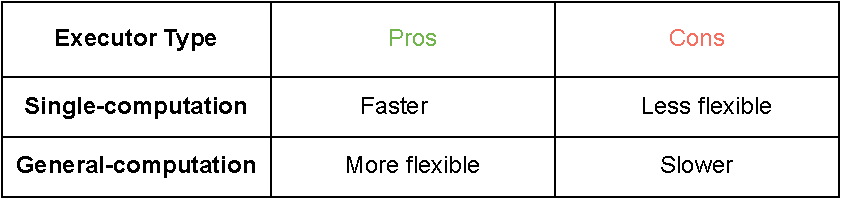
\includegraphics[scale=0.7]{\zkevmdir/figures/architecture/intro-proving-system/single-vs-general.drawio}
\end{figure}
\begin{itemize}
\small
\item The single-computation executor is faster because it does not need
to read assembly, it can implement the generation of the execution trace for the computation and
this process can be optimized for this computation.
\item However, the single-computation executor is not easy to change, test or audit.
\item In zkEVM we will have both, each one serving different purposes.
\item The single-computation executor is WIP.
\end{itemize}
\end{frame}




\begin{frame}[fragile]{zkASM: Assembly Language for the zkEVM}
\begin{itemize}

\item \textbf{zkASM} is the language developed by the team that is used to write the program that a compiler will build and the executor will interpret in order to build the execution trace.

\vspace{1em}

\begin{figure}
\begin{zkasm}
STEP => A
0                                   :ASSERT ; Ensure it is the beginning of the execution

CTX                                 :MSTORE(forkID)
CTX - %FORK_ID                      :JMPNZ(failAssert)

B                                   :MSTORE(oldStateRoot)
\end{zkasm}
\textbf{zkASM} Language Example.
\end{figure}

\vspace{1em}

\item In the repository \href{https://github.com/0xPolygonHermez/zkasmcom-vscode}{\texttt{zkasmcom-vscode}} there is a syntax highlighter for VSCode.

%npx vsce package
%code --install-extension NAME.vsix
\end{itemize}
\end{frame}






\begin{frame}{The zkASM Compiler}

\begin{block}{zkASM Compiler}
We have implemented a \href{https://github.com/0xPolygonHermez/zkasmcom}{zkASM compiler} that reads a zkASM specification file and compiles it to an output file with the list steps and instructions which the executor will consume in order to compute the execution trace.
\end{block}

\begin{figure}

\includegraphics[width=0.65\columnwidth]{\zkevmdir/figures/architecture/intro-proving-system/zkasmcom-basic.drawio}
\end{figure}

\end{frame}







\begin{frame}{ROM-based Executor}
\begin{itemize}
\item We need a \textbf{general-computation} executor because:
  \begin{itemize}
  \item Our implementation of the EVM evolves.
  \item The EVM itself also evolves.
  \end{itemize}

\item An architecture with assembly programs is faster to develop, test and audit than a specific implementation.

\item We call the Ethereum program that processes EVM transactions the \textbf{EVM ROM} (Read Only Memory) or simply the \textbf{ROM}.
\end{itemize}
\end{frame}




\begin{frame}{\texttt{forkId}}
\begin{itemize}
\item By changing the ROM, we make our L2 zkEVM more and more closer to the L1 EVM.
\item So we have versions of the zkEVM ROM.
\item Each of these versions will be denoted with an identifier called
\texttt{forkId}.
\item Another advantage of using a ROM-based approach is that we can test small parts of the assembly program
in isolation.
\item Finally, mention that:
  \begin{itemize}
  \item We are also developing a native executor (we will see why later).
  \item Having the two approaches allows us to check that execution traces generated match.
  \end{itemize}
\end{itemize}
\end{frame}




\ifARCHMAP
\begin{frame}{List of To Be Covered Concepts}
\begin{columns}
\begin{column}{0.48\textwidth}
\begin{itemize}
\item Provers. \hfill \CheckedBox
\item Execution trace. \hfill \CheckedBox
\item Witness and fixed columns. \hfill \CheckedBox
\item Executors (general purpose and computation-specific). \hfill \CheckedBox
\item zk Assembly. \hfill \CheckedBox
\item ROM of the zkEVM. \hfill \CheckedBox
\item forkId. \hfill \CheckedBox
\end{itemize}
\end{column}
\begin{column}{0.48\textwidth}
\begin{itemize}
\item PIL (Polynomial Identity Language). \hfill \Square
\item PIL2 (WIP). \hfill \Square
\item Publics and privates. \hfill \Square
\item Verifiers (Fflonk). \hfill \Square
\item Selector columns. \hfill \Square
\item zkEVM compatibility/equivalence types. \hfill \Square
\item Secondary execution matrices A.K.A state machines. \hfill \Square
\item PIL namespaces. \hfill \Square
\item State machine interconnection with lookups. \hfill \Square
\end{itemize}
\end{column}
\end{columns}
\end{frame}
\fi



\begin{frame}{Execution Correctness}
The execution correctness is enforced by a set of constraints that must be fulfilled by the execution trace:

\vspace{1em}
\begin{columns}[t]
\begin{column}{0.2\columnwidth}
\centering
\textbf{Program (computation): $(x_0+x_1)\cdot 4]\cdot x_2$} \\
\vspace{1em}
\begin{tabular}{|c|c|c|}
\hline
\textbf{A} & \textbf{B} & \cellcolor{lightgray} \textbf{C} \\ \hline
1 & 2 & \cellcolor{lightgray} \\ \hline
3 & & \cellcolor{lightgray} 4 \\ \hline
12 & 5 & \cellcolor{lightgray} \\ \hline
60 & & \cellcolor{lightgray} \\ \hline
\end{tabular}
\end{column}

\begin{column}{0.5 \columnwidth}
\centering
\vspace{-.5em}
\textbf{Constraints:}
\begin{align*}
&a_0 = x_0 \\
&b_0 = x_1 \\
&a_1 = a_0 + b_0 \\
&a_2 = a_1 \cdot 4 \\
&b_2 = x_2 \\
&a_3 = a_2 \cdot b_2
\end{align*}
\end{column}
\end{columns}
\end{frame}





\begin{frame}{The PIL Language and its Compiler}
\begin{itemize}
\item In our cryptographic backend:
  \begin{itemize}
  \item Each column is transformed into a polynomial (of the degree the number of rows).
  \item Constraints are defined over these polynomials.
  \item We describe constraints using a language called \textbf{PIL (Polynomial Identity Language)}.
  \end{itemize}
\end{itemize}

\small
\begin{block}{PIL Compiler}
We have implemented a \href{https://github.com/0xPolygonHermez/pilcom}{PIL compiler} that reads a PIL specification file and compiles it to an output file with the list of constraints and a format that can be consumed by the prover.
\end{block}
\begin{figure}

\includegraphics[width=0.65\columnwidth]{\zkevmdir/figures/architecture/intro-proving-system/pilcom-basic.drawio}
\end{figure}
\begin{itemize}
\item The repository \href{https://github.com/0xPolygonHermez/pilcom-vscode}{\texttt{pilcom-vscode}} contains a PIL syntax highlighter for VSCode.
\end{itemize}
\ifPROF
\footnotesize
\textbf{++Prof:} Latter we will see some PIL, but comment that a PIL specification can have a loop and the compiler
outputs the list of constraints which is what the prover in fact needs.
\normalsize
\fi
\end{frame}






\begin{frame}[allowframebreaks]{Publics and Privates}
\begin{itemize}
\item With zk-technology, we can create execution traces
where some of the inputs are \textbf{private}.
\vspace{0.3cm}
\begin{columns}
\begin{column}{0.33\textwidth}
\textbf{Example 1} \centering
$$
\begin{array}{|c|c|c|}
\hline
\textbf{A} & \textbf{B} & \cellcolor{lightgray} \textbf{C} \\ \hline
1 \cellcolor{green} & 2 \cellcolor{green}
& \cellcolor{lightgray} \\ \hline
3 & & 4 \cellcolor{lightgray} \\ \hline
12 & 5 \cellcolor{green} &
\cellcolor{lightgray} \\ \hline
60 \cellcolor{green} & & \cellcolor{lightgray}
\\ \hline
\end{array}$$
\end{column}
\begin{column}{0.33\textwidth}
\textbf{Example 2} \centering
$$
\begin{array}{|c|c|c|}
\hline
\textbf{A} & \textbf{B} & \cellcolor{lightgray} \textbf{C} \\ \hline
1 \cellcolor{green} & 2 \cellcolor{orange} &
\cellcolor{lightgray} \\ \hline
3 & & 4 \cellcolor{lightgray} \\ \hline
12 & 5 \cellcolor{green} &
\cellcolor{lightgray} \\ \hline
60 \cellcolor{green} & &
\cellcolor{lightgray} \\ \hline
\end{array}$$
\end{column}
\begin{column}{0.33\textwidth}
$\begin{array}{|c|}
\hline
\cellcolor{green}\\ \hline
\end{array}$
: publics \\ \vspace{0.2cm}
$\begin{array}{|c|} \hline
\cellcolor{orange}\\ \hline
\end{array}$
: privates \\ \vspace{0.2cm}
$\begin{array}{|c|} \hline
\cellcolor{lightgray}\\ \hline
\end{array}$
: fixed
\end{column}
\end{columns}
\vspace{0.3cm}
\item Recall that columns A and B are \textbf{witness} while the C column is
\textbf{fixed}.
\end{itemize}


\framebreak
\begin{columns}
\begin{column}{0.48\textwidth}
$$
\begin{array}{|c|c|c|}
\hline
\textbf{A} & \textbf{B} & \cellcolor{lightgray} \textbf{C} \\ \hline
1 \cellcolor{green} & 2 \cellcolor{orange} &
\cellcolor{lightgray} \\ \hline
3 & & 4 \cellcolor{lightgray} \\ \hline
12 & 5 \cellcolor{green} &
\cellcolor{lightgray} \\ \hline
60 \cellcolor{green} & &
\cellcolor{lightgray} \\ \hline
\end{array}$$
\end{column}
\begin{column}{0.48\textwidth}
\begin{itemize}
\item \textbf{Public inputs}: \{1, 5\}
\item \textbf{Private inputs}: \{2\}
\item \textbf{Output (public)}: \{60\}
\item \textbf{Publics}: \{{1, 5, 60}\}
\end{itemize}
\end{column}
\end{columns}

\vspace{0.5cm}
In this execution trace design, input $x_1$ is
private, while inputs $x_0$ and $x_2$ are public and
the output is also public.

\vspace{0.1cm}
Publics are enforced by constraints.
\end{frame}




\begin{frame}{Generating and Verifying Proofs}
\begin{figure}[H]
\centering
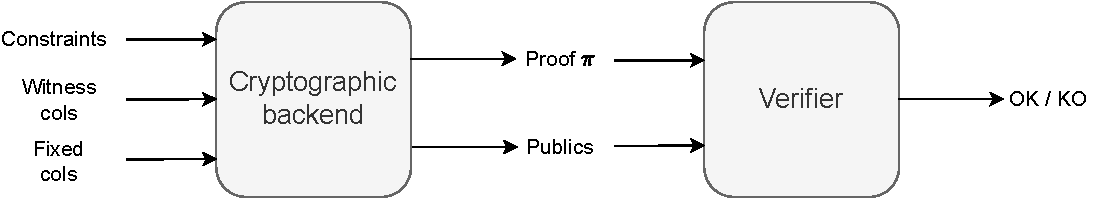
\includegraphics[scale=0.65]{\zkevmdir/figures/architecture/intro-proving-system/generating-verifying-proofs.drawio}
\end{figure}
\begin{itemize}
\small
\item With a valid proof $\pi$, the verifier is convinced that
the execution of the computation in question is correct for the given public inputs.

\item $\pi$ is small and needs a small amount of
resources to be validated.
\item In our case, currently we use a backend cryptographic system whose final verifier is \textbf{FFlonk}.
\item \textbf{Note}: A smart contract in the L1 execution layer can verify the proof implementing a FFlonk verifier (and therefore validate the computation of a new state from a batch) with $\approx 200K$ gas.
\end{itemize}
\end{frame}



\begin{frame}[fragile]{Example of Usage of a Private Input}

A typical example of using a private input is to prove the knowledge of
the pre-image of a hash without revealing this pre-image value:

\begin{figure}
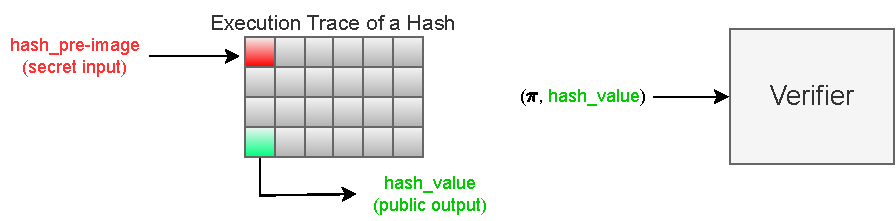
\includegraphics[width=0.9\columnwidth]{\zkevmdir/figures/architecture/intro-proving-system/private-input-hash-example.drawio}
\end{figure}

\ifPROF
\vspace{0.2cm}
\scriptsize
\textbf{++Prof:} We can show some variants with a concatenation of another public input value.
\normalsize
\fi

\end{frame}







\begin{frame}{Shaping Execution Traces}
\begin{itemize}
\item In an execution trace, each row is in charge of validating an \textbf{zkASM operation} or \textbf{part of an operation}.
\item For example, suppose that we are given a set of $3$ operations \texttt{OP1, OP2} and \texttt{OP3}.
\item These operations change the next\footnote{Primes mean next value of some column, e.g. $a'$ means the next value in the \textbf{A} column.}
value of the \textbf{A} column.
\begin{align*}
&\texttt{OP1}: a'=a+b+c \\
&\texttt{OP2}: a'=a+b+c+d+e\\
&\texttt{OP3}: a'=a+b+c+d+e+f+g+h
\end{align*}
\item Consider also that we have an execution trace matrix of $6$ columns.

\vspace{0.1cm}
\begin{columns}
\begin{column}{0.4 \textwidth}

\scriptsize

\begin{table}[h!]
\begin{tabular}{|c|c|c|c|c|c|}
\hline
\textbf{A} & \textbf{B} & \textbf{C} & \textbf{D} & \textbf{E} & \textbf{F} \\ \hline
 &  &  & & &\\ \hline
 &  &  &  &  &  \\ \hline
 &  &  &  &  & \\ \hline
 &  &  &&& \\ \hline
\end{tabular}
\end{table}
\end{column}
\begin{column}{0.36 \textwidth}
\item \textbf{Q.} Can we fit this computation inside the matrix? how?
\end{column}
\end{columns}
\vspace*{5mm}
\end{itemize}
\end{frame}





\begin{frame}{Shaping Execution Traces: Strategies}
\begin{itemize}
\item We can adopt two straightforward strategies:
  \begin{enumerate}[a)]
  \item Increasing the number of columns so that we can fit every summand.
  \item Use the next row in order to fit some of the remaining summands of the operation.
  \end{enumerate}

\vspace{1em}

\item Using the second approach, we can define an execution matrix in which \texttt{OP3}
uses two rows:
\begin{align*}
&\texttt{OP1}: a'=a+b+c \\
&\texttt{OP2}: a'=a+b+c+d+e\\
&\texttt{OP3}: a'=a+b+c+d+e+f+b'+c'
\end{align*}

\scriptsize
\vspace{1em}

\begin{table}[h!]
\begin{tabular}{|c|c|c|c|c|c|}
\hline
\textbf{A} & \textbf{B} & \textbf{C} & \textbf{D} & \textbf{E} & \textbf{F} \\ \hline
$a_0$ & $b_0$ & $c_0$ & & &\\ \hline
$a_1$ & $b_1$ & $c_1$ & $d_1$ & $e_1$ & \\ \hline
\cellcolor{yellow} $a_2$ & \cellcolor{yellow} $b_2$ & \cellcolor{yellow}  $c_2$ & \cellcolor{yellow} $d_2$ & \cellcolor{yellow} $e_2$ & \cellcolor{yellow} $f_2$ \\ \hline
\cellcolor{green} $a_3$ & \cellcolor{yellow}  $b_3$ & \cellcolor{yellow}  $c_3$ &&& \\ \hline
\end{tabular}
\hspace{1em}
\begin{tabular}{c}
              \\
$\mathtt{OP1}$ \\
$\mathtt{OP2}$ \\
$\mathtt{OP3}$ \\
$             $ \\
\end{tabular}
\end{table}
\end{itemize}
\end{frame}






\begin{frame}[allowframebreaks]{Execution Trace Design Strategies}
Number of rows and columns?

\vspace{0.25cm}
\begin{itemize}
\item The maximum number of rows might be fixed by a cryptographic back-end
(this is the case of our current back-end).
\item The fewer rows used, the faster the prover is.
\item In practice, $\# rows=2^n$ for some natural $n \in \mathbb{N}$.
\item More or less columns?  Adding columns also increases proving time.
\end{itemize}


\framebreak
\begin{columns}
\begin{column}{0.48\textwidth}
\begin{table}[h!]
\begin{tabular}{c}
$             $ \\
$\mathtt{OP1}$ \\
$\mathtt{OP2}$ \\
$             $
\end{tabular}
\begin{tabular}{|c|c|c|c|c|c|}\hline
$\mathbf{A}$ & $\mathtt{B}$ & $\mathtt{C}$ & $\mathtt{D}$ & $\mathtt{E}$ & $\mathtt{F}$ \\ \hline
$a_0$ & $b_0$ & $c_0$ & \cellcolor{cyan} & \cellcolor{cyan} & \cellcolor{cyan} \\ \hline
$a_1$ & $b_1$ & $c_1$ & $d_1$ & $e_1$ & \cellcolor{cyan} \\ \hline
\cellcolor{green} $a_2$ & \cellcolor{cyan} & \cellcolor{cyan} & \cellcolor{cyan} & \cellcolor{cyan} & \cellcolor{cyan} \\ \hline
\end{tabular}
\end{table}
\vspace{0.3cm}
\end{column}
\begin{column}{0.48\textwidth}
\texttt{OP1}: $a'=a+b+c$
\\ \texttt{OP2}: $a'=a+b+c+d+e$
\\ \textit{$6$ columns and $3$ rows.}
\\ \textit{$18$ cells but $9$ of them unused.}
\end{column}
\end{columns}
\begin{columns}
\begin{column}{0.48\textwidth}

\vspace{0.2cm}
\begin{table}[h!]
\begin{tabular}{c}
$             $ \\
$\mathtt{OP1}$ \\
$\mathtt{OP2}$ \\
$             $
\end{tabular}
\begin{tabular}{|c|c|c|}\hline
$\mathbf{A}$ & $\mathtt{B}$ & $\mathtt{C}$ \\ \hline
$a_0$ & $b_0$ & $c_0$ \\ \hline
$a_1$ & $b_1$ & $c_1$ \\ \hline
$a_2$ & $b_2$ & \cellcolor{green}$c_2$ \\ \hline
\end{tabular}
\end{table}
\end{column}
\begin{column}{0.48\textwidth}
\texttt{OP1}: $a'=a+b+c$
\\ \texttt{OP2}: $c'=a+b+c+a'+b'$
\\ \textit{$3$ columns and $3$ rows.}
\\ \textit{$9$ cells and all of them used. }
\end{column}
\end{columns}
\#unused\_cells depends on the instructions executed and the execution matrix shape.
\end{frame}





\begin{frame}{Selector Columns}
\begin{columns}
\begin{column}{0.48\textwidth}
\begin{table}[h!]
\begin{tabular}{c}
$             $ \\
$\mathtt{OP1}$ \\
$\mathtt{OP2}$ \\
$             $
\end{tabular}
\begin{tabular}{|c|c|c|}\hline
$\mathbf{A}$ & $\mathtt{B}$ & $\mathtt{C}$ \\ \hline
$a_0$ & $b_0$ & $c_0$ \\ \hline
$a_1$ & $b_1$ & $c_1$ \\ \hline
$a_2$ & $b_2$ & $c_2$ \\ \hline
\end{tabular}
\end{table}
\end{column}
\begin{column}{0.48\textwidth}
\texttt{OP1}: $a+b+c-a'=0$
\\ \texttt{OP2}: $a+b+c+a'+b'-c'=0$
\end{column}
\end{columns}


\begin{itemize}
\small
\item Since we are using constraints with columns (not cells), we need to add \textbf{selector columns}.
\item Selector columns are used to control wether the constraints apply or not (meaning whether we are performing this or that operation).
\end{itemize}

\begin{columns}
\begin{column}{0.48\textwidth}
\begin{table}[h!]
\begin{tabular}{c}
$             $ \\
$\mathtt{OP1}$ \\
$\mathtt{OP2}$ \\
$             $
\end{tabular}
\begin{tabular}{|c|c|c|c|c|}\hline
$\mathbf{A}$ & $\mathtt{B}$ & $\mathtt{C}$ & $\mathtt{OP1}$ & $\mathtt{OP2}$ \\ \hline
$a_0$ & $b_0$ & $c_0$ & 1 & 0 \\ \hline
$a_1$ & $b_1$ & $c_1$ & 0 & 1\\ \hline
$a_2$ & $b_2$ & $c_2$ & & \\ \hline
\end{tabular}
\end{table}
\end{column}
\begin{column}{0.48\textwidth}
\begin{align*}
op1*(1-op2)*(a+b+c-a') &+  \\
op2*(1-op1)*(a+b+c+a'+b'-c') &= 0
\end{align*}
\end{column}
\end{columns}
\end{frame}





\begin{frame}{The Execution Trace and the zkEVM}
\begin{itemize}
\small
\item In our current cryptographic backend, we have a shape that is pre-fixed for the execution trace.
\item Also, we don't know exactly what EVM opcodes (and as a consequence zkEVM operations) will be executed, 
since this depends on the particular transactions of the L2 batch.
\item The pre-fixed shape fixes in turn the amount of computation that we can do, which
in our case is the amount and type of L2 transactions for which we can generate a proof.
\item  In general, it is hard to optimize the shape of a single execution trace matrix:
\end{itemize}
\begin{columns}
\begin{column}{0.36\textwidth}
\begin{enumerate}
\footnotesize
\item \textbf{Narrow matrices may easily hit the max row limit}, which is about $2^{23}$
(fixed by the cryptographic back-end).
\item \textbf{Wide matrices might be inefficient} for mixing many different instructions.
\end{enumerate}
\end{column}
\begin{column}{0.55\textwidth}
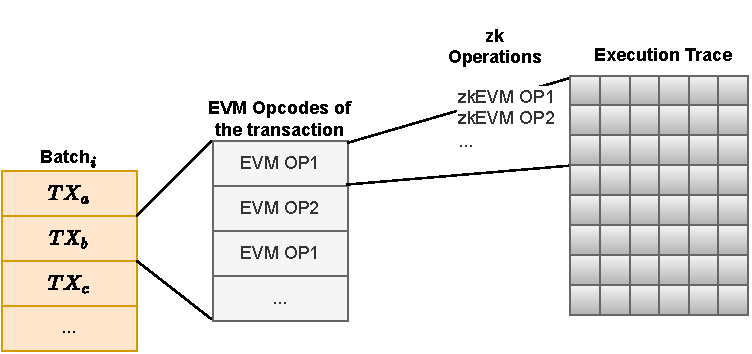
\includegraphics[width=\columnwidth]{\zkevmdir/figures/architecture/intro-proving-system/batch-evmopcode-zkop-trace.drawio}
\end{column}
\end{columns}
\end{frame}




\begin{frame}[fragile, allowframebreaks]{zkEVMs Compatibility/Equivalence}
\begin{columns}
\begin{column}{0.46\textwidth}
\begin{itemize}
\footnotesize
\item A layer 2 is EVM compatible or equivalent if it can run EVM byte code without modifying the underlying smart contract logic. 
\item EVM compatibility allow L2's to use existing Ethereum smart contracts, patterns, standards, and tooling.
\item Being EVM compatible is important for the widespread adoption of these L2 since this allows using existing tools can be used.
\item In practice, there are several types of compatibility.
\item \textbf{Type 1:} Fully Ethereum equivalent, i.e. they do not change any part of the Ethereum system but generating proofs
can take several hours.
\end{itemize}
\end{column}
\begin{column}{0.51\textwidth}
\begin{itemize}
\footnotesize
\item \textbf{Type 2:} Fully EVM-equivalent, but changes some different internal representations like how they store the state of the chain, for the purpose of improving ZK proof generation times.
\item \textbf{Type 2.5:} Fully EVM-equivalent, except they use different gas costs for some operations to "significantly improve worst-case prover times".
\item \textbf{Type 3:} Almost EVM-equivalent zkEVMs make sacrifices in exact equivalence to further enhance prover times and simplify EVM development.
\item \textbf{Type 4:} High-level language equivalent zkEVMs compile smart contract source code written in a high-level language to a friendly language for zk, resulting in faster prover times but potentially introducing incompatibilities and limitations.
\end{itemize}
\end{column}
\end{columns}




\framebreak
\begin{figure}
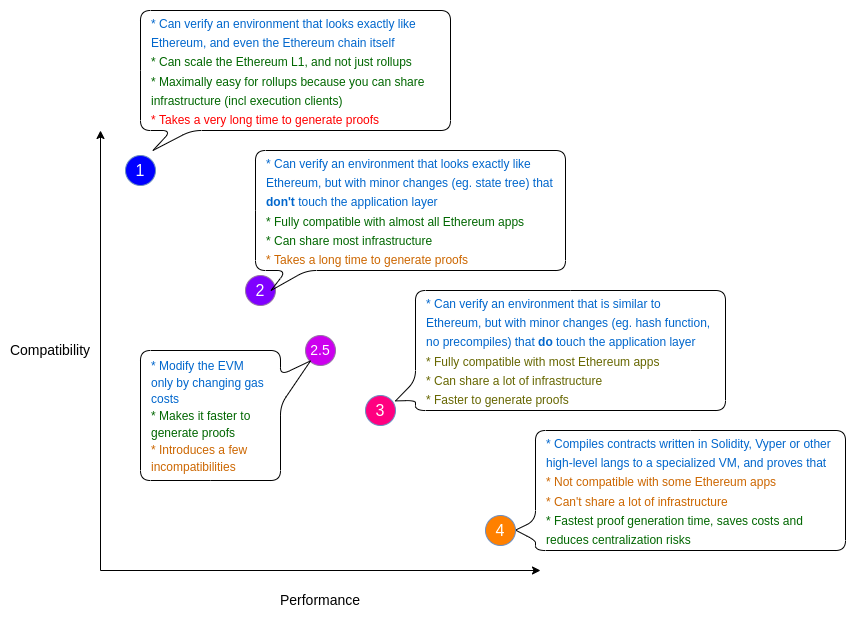
\includegraphics[width=0.6\columnwidth]{\zkevmdir/figures/architecture/intro-proving-system/zkEVM-compatibility-post-vitalik}
\footnotesize
\url{https://vitalik.ca/general/2022/08/04/zkevm.html}
\end{figure}
\end{frame}






\begin{frame}{Motivational Example: Implementing an EXP Operation}
\begin{itemize}
\small
\item Let's assume that our cryptographic backend only allows to define constraints with additions and multiplications.
\item Let's consider also that we want to implement a exponentiation operation (\texttt{EXP}).
\item Then, we can use several rows doing multiplications to implement \texttt{EXP}.
\item A portion of the execution trace (that implements $2^5 = 32$) could be:
\begin{columns}
\begin{column}{0.2\textwidth}
$$
\begin{array}{|c|c|c|}
\hline
\textbf{A} & \textbf{B} & \textbf{C} \\ \hline
2 & 5 & 2  \\ \hline
2 & 4 & 4  \\ \hline
2 & 3 & 8  \\ \hline
2 & 2 & 16 \\ \hline
2 & 1 & 32 \\ \hline
\end{array}$$
\end{column}

\begin{column}{0.7\textwidth}
\small
An incomplete (\textbf{uncorrected}) set of constraints:

\vspace{0.1cm}
\begin{enumerate}
\small
\item $a'=a$ \quad 
(the \textbf{A} column represents the base)
\item $b'=b-1$ \quad 
(the \textbf{B} column stores the decreasing exponent)
\item $c'=c\cdot a$ \quad 
(the \textbf{C} column stores the intermediate results)
\end{enumerate}
\end{column}
\end{columns}

\vspace{0.2cm}
\item If we want to implement this operation in the main Execution Trace, note that
we are going to spend several rows per \texttt{EXP} operation.
\item In fact, a variable number of rows per \texttt{EXP} operation depending on the exponent.
\end{itemize}
\end{frame}










\begin{frame} {Secondary Execution Trace Matrices and Lookup Arguments}
\begin{itemize}
\item The previous approach leads to a very complicated set of constraints together with a huge amount
of consumed rows by operations, which is quite an unwanted scenario.
\item Another approach is to use \textbf{tailor-made secondary execution traces for specific operation(s)}:
  \begin{itemize}
  \item In this approach, there is a \textbf{main execution trace} and there are also \textbf{secondary execution traces}.
  \item In the cryptographic back-end, we use a mechanism called \textbf{lookup argument} to \textbf{link} these execution trace matrices.
  \item In particular, the lookup argument provides the constraints necessary to check that certain cells of a row in an execution trace matrix match other cells in a row of another execution trace matrix.
  \end{itemize}
\item So, another approach for our \texttt{EXP} operation is to implement it in a secondary execution trace matrix
and link the main execution trace with the secondary trace with a \textbf{lookup argument}.
\end{itemize}
\end{frame}





\begin{frame}{Main Trace with Delegated Operation checks}
\begin{columns}
\begin{column}{0.3\textwidth}
$$\begin{array}{|c|c|c|c|}
\hline
\textbf{A} &  \textbf{B} & \textbf{C} &  \textbf{EXP}\\ \hline
\cdots & \cdots & \cdots & 0 \\ \hline
2 & 5 & 32 & 1 \\ \hline
\cdots & \cdots & \cdots & 0 \\ \hline
\cdots & \cdots & \cdots & 0 \\ \hline
\cdots & \cdots & \cdots & 0 \\ \hline
\cdots & \cdots & \cdots & 0 \\ \hline
3 & 2 & 9 & 1 \\ \hline
\cdots & \cdots & \cdots & 0 \\ \hline
\cdots & \cdots & \cdots & 0 \\ \hline
& & & \\ \hline
\end{array} $$
\end{column}
\begin{column}{0.7\textwidth}
\begin{itemize}
\item In the main execution trace, each \texttt{EXP} operation occupies
just one row.
\item Notice that we introduced the \textbf{EXP} selector to indicate
when the \texttt{EXP} operation is being performed.
\item For the first \texttt{EXP} operation, inputs are 2
and 5 and the result is 32.
\item The correctness of the result will be
validated in a secondary execution matrix.
\end{itemize}
\end{column}
\end{columns}
\end{frame}




\begin{frame}{State Machine (SM) Concept and Lookup Between SMs}
\begin{columns}
\begin{column}{0.35\textwidth}
\begin{itemize}
\item An execution trace matrix can be seen as a
set of states (\textbf{state machine}), in which
each row is a state.
\item We will use both, the terms "execution trace matrix" and "state machine" interchangeably.
\end{itemize}
\end{column}
\begin{column}{0.3\textwidth}
\textbf{Main state machine} \centering

\vspace{-0.7cm}
$$ \begin{array}{|c|c|c|c|}
\hline
\textbf{A} &  \textbf{B} & \textbf{C} &  \textbf{EXP}\\
\hline
\cdots & \cdots & \cdots & 0 \\ \hline
2  \cellcolor{yellow} & 5 \cellcolor{yellow} &
32 \cellcolor{yellow} & 1 \cellcolor{yellow} \\
\hline
\cdots & \cdots & \cdots & \cdots \\ \hline
3  \cellcolor{yellow} & 2 \cellcolor{yellow} & 9
\cellcolor{yellow} & 1 \cellcolor{yellow} \\ \hline
\cdots & \cdots & \cdots & 0 \\ \hline
\end{array} $$
\begin{flushleft} \hspace{0.6cm}
$ \begin{array}{|c|}
  \hline \cellcolor{yellow} \\ \hline
\end{array}$
: Lookup
\end{flushleft}
\end{column}
\begin{column}{0.3\textwidth}
\textbf{EXP state machine} \centering

\vspace{-0.7cm}
$$\begin{array}{|c|c|c|c|c|}
\hline
\textbf{A} & \textbf{B} & \textbf{C} & \textbf{D}
& \textbf{EXP} \\ \hline
2 & 5 & 2 & 5 & 0 \\ \hline
2 & 5 & 4 & 4 & 0 \\ \hline
2 & 5 & 8 & 3 & 0 \\ \hline
2 & 5 & 16 & 2 & 0 \\ \hline
2 \cellcolor{yellow} & 5 \cellcolor{yellow} &
32 \cellcolor{yellow} & 1 & 1
\cellcolor{yellow}\\ \hline
3 & 2 & 3 & 2 & 0 \\ \hline
3 \cellcolor{yellow} & 2 \cellcolor{yellow} & 9
\cellcolor{yellow} & 1 & 1 \cellcolor{yellow} \\ \hline
& & & & \\ \hline
\end{array} $$
\end{column}
\end{columns}

\vspace{0.2cm}
\begin{itemize}
\item Constraints in the secondary SM enforce the
correctness of the \texttt{EXP} operation.
\item In the main SM, we just put the inputs/outputs,
that we call \textit{"free"}, in a single row.
\end{itemize}
\end{frame}








\ifPILFOURBYTEEXAMPLE
\begin{frame}[fragile]{Example: Byte4 SM}
\begin{columns}
\begin{column}{0.5\textwidth}
\[
\begin{array}{|a|c|c|c|}
\hline
\textbf{SET} &  \textbf{free} & \textbf{out} &  \textbf{out'}\\ \hline
0 & $\textsf{0xba04}$ & \cellcolor{black} \color{white} \mathbf{0x00000000} & $\textsf{0x0000ba04}$ \\ \hline
1 & $\textsf{0x3ff2}$ & \cellcolor{black} \color{white} \mathbf{0x0000ba04} & $\textsf{0xba043ff2}$ \\ \hline
0 & $\textsf{0x4443}$ & \cellcolor{black} \color{white} \mathbf{0xba043ff2} & $\textsf{0x00004443}$ \\ \hline
1 & $\textsf{0xc1d1}$ & \cellcolor{black} \color{white} \mathbf{0x00004443} & $\textsf{0x4443c1d1}$ \\ \hline
0 & $\textsf{0xd11e}$ & \cellcolor{black} \color{white} \mathbf{0x4443c1d1} & $\textsf{0x0000d11e}$ \\ \hline
1 & $\textsf{0x6ab9}$ & \cellcolor{black} \color{white} \mathbf{0x0000d11e} & $\textsf{0xd11e6ab9}$ \\ \hline
0 & \cdots          & \cellcolor{black} \color{white} \mathbf{0xd11e6ab9} & \cdots   \\ \hline
\cdots & \cdots & \cdots & \cdots    \\ \hline
\end{array}
\]
\end{column}
\begin{column}{0.5\textwidth}
\begin{itemize}
\item In one row (also named clock), the first 16-bit free input is moved to $\textsf{out}$.
\item In the following clock, the next 16-bit free input is moved+concatenated to $\textsf{out}$. 
\item We introduce the \texttt{SET} constant polynomial to manage the alternating move and move+concatenation.
\item Note that we have valid 32-bit numbers in the \texttt{out} column.
\end{itemize}
\end{column}
\end{columns}
\end{frame}








\begin{frame}[fragile]{Example: PIL for the Byte4 SM}
\begin{columns}
\begin{column}{0.5\textwidth}
\begin{itemize}
\item The computation is enforced with the following constraint:
\[
\textsf{out}' = (1 - \textsf{SET}) \cdot \textsf{free} + \textsf{SET} \cdot (2^{16} \cdot \textsf{out} + \textsf{free}).
\]
\end{itemize}
\begin{pil}
namespace Global(%N);
    pol constant L1;
    pol constant BYTE2; // [0,1,...,65535]

namespace Byte4(%N);
  pol constant SET; // [0, 1, 0, 1, 0, 1, ...]
  pol commit free;
  pol commit out;

  // Identities 
  free in Global.BYTE2; // Lookup: input in [0,...,65535]
  out' = (1 - SET)*free + SET*(2**16*out + free);
\end{pil}
\end{column}
\begin{column}{0.5\textwidth}
\begin{itemize}
\item Notice that when $\textsf{SET} = 0$, then $\textsf{out}' = \textsf{free}$, i.e., $\textsf{out}$ is set to be the first input. 
\item In contrast, when $\textsf{SET} = 1$, then $\textsf{out}' = 2^{16} \cdot \textsf{out} + \textsf{free}$, i.e., the previous input (stored in $\textsf{out}$) is set to be the upper part of $\textsf{out}$, while the second input is set to be the lower part of $\textsf{out}$. 
\item To achieve soundness, we must also check that both free inputs are numbers of $2$ bytes.
\end{itemize}
\end{column}
\end{columns}

\ifPROF
\vspace{0.2cm}
\scriptsize
\textbf{++Prof:}
\$ node ../../pilcom/src/pil.js example.pil -o output.pil.json
\normalsize
\fi
\end{frame}
\fi




\begin{frame}{The PIL of the zkEVM}
\begin{itemize}
\item Recall that there is a \href{https://github.com/0xPolygonHermez/pilcom}{PIL compiler} that reads a PIL specification file and compiles it to an output file with the list of constraints and a format that can be consumed by the prover.
\item In the PIL language, the state machines (subexecution matrices) are called \texttt{namespaces}.
\item In the \href{https://github.com/0xPolygonHermez/zkevm-proverjs}{zkevm-proverjs} repository, you can find the \href{https://github.com/0xPolygonHermez/zkevm-proverjs/tree/main/pil}{PIL specification of the zkEVM} under the pil directory.
\end{itemize}

\ifPROF
\vspace{0.2cm}
\footnotesize
\textbf{++Prof:} 

- In the PIL compiler README explain namespaces and trace size.

- Show PIL of the zkEVM: lookups, publics and some constraints.
\fi
\end{frame}




\begin{frame}{Remarks about the Computation and the Shape of SMs}
\begin{columns}
\begin{column}{0.48 \textwidth}
\begin{itemize}
\small
\item The columns of each state machine are defined by
the design of its corresponding execution trace.
\item Due to limitations of our current cryptographic backend, all the SM must have the same number of rows.
\item The computation of an L2 batch can have branches and loops and hence, 
each L2 batch execution can use a different number of operations in the zkEVM.
\item As a result, the number of rows used at each SM depends on the
number of operations of each type during the batch execution.
\end{itemize}
\end{column}

\begin{column}{0.5 \textwidth}
\begin{itemize}
\small
\item Since the number of rows is fixed (and the same for all State Machines) we
can have \textit{unused} rows.
\item But, what is more important is that obviously, \textbf{the size of the computation being proved must fit 
in the execution trace matrices available}.
\end{itemize}
\begin{figure}
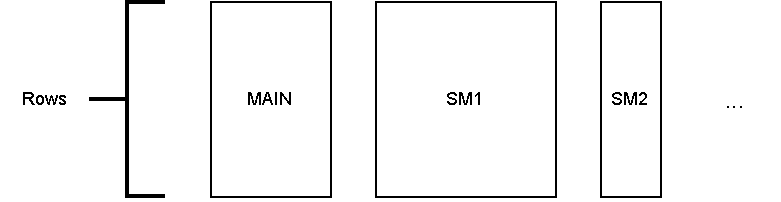
\includegraphics[width=\columnwidth]{\zkevmdir/figures/architecture/intro-proving-system/shape-state-machines.pdf}
\end{figure}

\ifPROF
\vspace{0.2cm}
\scriptsize
\textbf{++Prof:} Draw in the picture when we have unused rows and a possible overflow.
\normalsize
\fi

\end{column}
\end{columns}
\end{frame}



%TODO WIP
\begin{frame}{PIL Evolution: PIL2 (WIP)}
\begin{itemize}
\item Currently, we are under the development of a new version of PIL called \textbf{PIL2}.

\vspace{0.2cm}
\item PIL2 is designed to operate with a more powerful cryptographic backend that is able to 
generate as many subexecution traces as required by the batch processing so that we never run out of rows.

\vspace{0.2cm}
\item We are also agreeing with the rest of the "zk projects" at Polygon a format for the PIL output file called "pilout".
\end{itemize}
\end{frame}





\begin{frame} {Recap of the Prover}
\begin{figure}
\centering
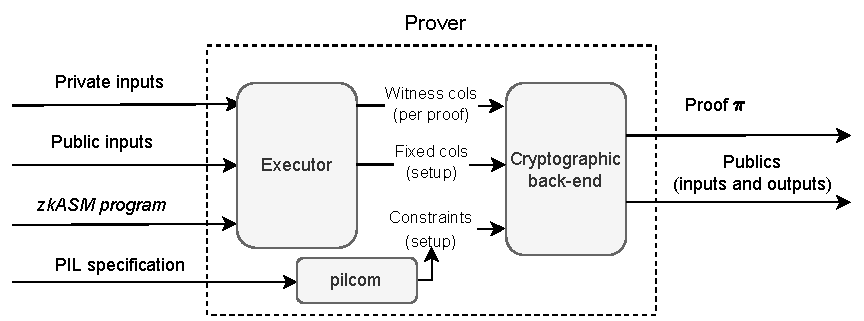
\includegraphics[width=0.95\columnwidth]{\zkevmdir/figures/architecture/intro-proving-system/prover-diagram.drawio}
\end{figure}

\footnotesize
\textbf{Note.} The files containing the pre-processed fixed columns and the processed witness columns for the zkEVM are temporary stored in binary files and are quite large (>100Gb).
\end{frame}



\begin{frame}{Recap of the Verifier}
\begin{itemize}
\item In our previous example:

\vspace{1em}

\begin{columns}
\begin{column}{0.40\textwidth}
$$
\begin{array}{|c|c|c|} \hline
\textbf{A} & \textbf{B} & \cellcolor{lightgray} \textbf{C} \\ \hline
1 \cellcolor{green} & 2 \cellcolor{orange} & \cellcolor{lightgray} \\ \hline
3 & & 4 \cellcolor{lightgray} \\ \hline
12 & 5 \cellcolor{green} & \cellcolor{lightgray} \\ \hline
60 \cellcolor{green} & & \cellcolor{lightgray} \\ \hline
\end{array}
$$
\end{column}

\begin{column}{0.26\textwidth}
$ \begin{array}{|c|} \hline \cellcolor{green}\\ \hline \end{array} $
: publics \\ \vspace{0.2cm}
$ \begin{array}{|c|} \hline \cellcolor{orange}\\ \hline \end{array} $
: privates \\ \vspace{0.2cm}
$ \begin{array}{|c|} \hline \cellcolor{lightgray}\\ \hline\end{array}$
: fixed
\end{column}
\begin{column}{0.33\textwidth}
\begin{itemize}
\item \textbf{Public inputs}: \{1, 5\}
\item \textbf{Private inputs}: \{2\}
\item \textbf{Output} (public): \{60\}
\item \textbf{Publics}: \{{1, 5, 60}\}
\end{itemize}
\end{column}
\end{columns}
\vspace{0.3cm}
\item Then the verifier:
\end{itemize}
\begin{figure}[H]
\centering
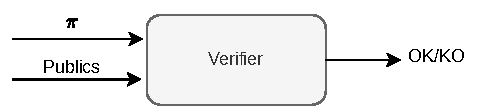
\includegraphics[width=0.6\columnwidth]{\zkevmdir/figures/architecture/intro-proving-system/verifier-diagram}
\end{figure}
\end{frame}






\ifARCHMAP
\begin{frame}{List of Covered Concepts}
\begin{columns}
\begin{column}{0.48\textwidth}
\begin{itemize}
\item Provers. \hfill \CheckedBox
\item Execution trace. \hfill \CheckedBox
\item Witness and fixed columns. \hfill \CheckedBox
\item Executors (general purpose and computation-specific). \hfill \CheckedBox
\item zk Assembly. \hfill \CheckedBox
\item ROM of the zkEVM. \hfill \CheckedBox
\item forkId. \hfill \CheckedBox
\item PIL (Polynomial Identity Language). \hfill \CheckedBox
\end{itemize}
\end{column}
\begin{column}{0.48\textwidth}
\begin{itemize}
\item PIL2 (WIP). \hfill \CheckedBox
\item Publics and privates. \hfill \CheckedBox
\item Verifiers (Fflonk). \hfill \CheckedBox
\item Selector columns. \hfill \CheckedBox
\item zkEVM compatibility/equivalence types. \hfill \CheckedBox
\item Secondary execution matrices A.K.A state machines. \hfill \CheckedBox
\item PIL namespaces. \hfill \CheckedBox
\item State machine interconnection with lookups. \hfill \CheckedBox
\end{itemize}
\end{column}
\end{columns}
\end{frame}
\fi

